\documentclass[letterpaper, 10 pt, conference]{ieeeconf}  % Comment this line out if you need a4paper
%\documentclass[a4paper, 10pt, conference]{ieeeconf}      % Use this line for a4 paper

\IEEEoverridecommandlockouts                              % This command is only needed if 
                                                          % you want to use the \thanks command
\overrideIEEEmargins                                      % Needed to meet printer requirements.

%In case you encounter the following error:
%Error 1010 The PDF file may be corrupt (unable to open PDF file) OR
%Error 1000 An error occurred while parsing a contents stream. Unable to analyze the PDF file.
%This is a known problem with pdfLaTeX conversion filter. The file cannot be opened with acrobat reader
%Please use one of the alternatives below to circumvent this error by uncommenting one or the other
%\pdfobjcompresslevel=0
%\pdfminorversion=4

% See the \addtolength command later in the file to balance the column lengths
% on the last page of the document

% The following packages can be found on http:\\www.ctan.org
\usepackage{graphicx} % for pdf, bitmapped graphics files
%\usepackage{epsfig} % for postscript graphics files
%\usepackage{mathptmx} % assumes new font selection scheme installed
%\usepackage{times} % assumes new font selection scheme installed
%\usepackage{amsmath} % assumes amsmath package installed
%\usepackage{amssymb}  % assumes amsmath package installed

\title{\LARGE \bf
Silver Spoon Effect on Education: Analysis of the effect of household wealth toward children's educational output
}


\author{Hyecheol Jang$^{*1}$, Carleigh Heintz$^{*2}$, Chang Su$^{*3}$, Desmond Fung$^{*4}$, and Tsz Yau Iris Chow$^{*5}$% <-this % stops a space
\thanks{$^{*}$Everyone is undergraduate student of the Department of  Statistics, University of Wisconsin - Madison (Madison, WI, 53706, USA), taking STAT 333 during FALL19, with professor Karl Rohe.}%
\thanks{$^{1}$Hyecheol Jang
        {\tt\small hyecheol.jang@wisc.edu}}%
\thanks{$^{2}$Carleigh Heintz
        {\tt\small cmheintz@wisc.edu}}%
\thanks{$^{3}$Chang Su
        {\tt\small csu29@wisc.edu}}%
\thanks{$^{4}$Desmond Fung
        {\tt\small dfung2@wisc.edu}}%
\thanks{$^{5}$Tsz Yau Iris Chow
        {\tt\small tchow7@wisc.edu}}%
}



\begin{document}

\maketitle
\thispagestyle{empty}
\pagestyle{empty}


%%%%%%%%%%%%%%%%%%%%%%%%%%%%%%%%%%%%%%%%%%%%%%%%%%%%%%%%%%%%%%%%%%%%%%%%%%%%%%%%
\begin{abstract}

This electronic document is a ÒliveÓ template. The various components of your paper [title, text, heads, etc.] are already defined on the style sheet, as illustrated by the portions given in this document.

\end{abstract}


%%%%%%%%%%%%%%%%%%%%%%%%%%%%%%%%%%%%%%%%%%%%%%%%%%%%%%%%%%%%%%%%%%%%%%%%%%%%%%%%
\section{INTRODUCTION}

Nowadays, the majority of countries and societies are having a hard-time addressing long-resting social issues: polarization.
Modern society rarely has an identifying system, but due to the extreme polarization, it is not difficult to see separated “classes”, classified people’s life-style by wealthiness, in the real world.
With the instinct of mankind, everyone wants to be a part of upper-class society, and they, especially middle and lower class households believe education could be a ladder to go up to the upper class.
According to Rugarber (2017, [1]), the higher-education degree holder gained about 1.5 times higher salary compared to those who only have a high-school diploma.
Also, by showing two sets of data with different time-frames, in the years 1999 and 2015, Rugarber was able to address that the wage gap becomes wider over time (para. 1-3).
Seeing the previous analysis of the data, it looks like the higher educational status makes a higher salary, which lets people move toward the upper class.

However, education opportunities are not equally provided for all people in this society.
With investment of additional resources on children’s education, paying tuition for private school, hiring tutors, and even sending their kids to other countries, people expect to bring better opportunity to their kids; therefore, education could be one of the ways to transfer the wealth of parents’ generation to their kids, making polarization even worse.
By conducting this research, we want to verify the existence of the "silver spoon effect" - if parents are wealthy, their kids are more likely to be wealthy - caused by education.
Specifically, we want to show that the areas with higher economic status and with the strong willingness of investing more on their next generations’ education have better educational output, expecting we can see a positive relationship between wealth and educational results (ACT Score, High School Graduation Rate, Statewide test score).

By showing the relatedness of wealth and educational output, we, ultimately, want to verify whether education might be used as a tool for “upper classes” to indirectly shift their capitals and superior societal position to the next generation.

\section{DATA COLLECTION / ANALYSIS}

Before going through how we collected and analyzed the datasets, note that all relevent dataset, codes, and documents are in our GitHub repository (URL: https://github.com/hyecheol123/STAT333-Edugression)

\subsection{Wisconsin Income by County}

Before analyzing the relationship between the economic status and the educational output, we started to make a graph of annual wage per employee for each county in Wisconsin.
This can be used gauge which citizens within the counties of the state are making more money compared to others, we are using this as a proxy variable for economic status.

The data has been retrieved from Bureau of Labor Statics (BLS)'s "Quarterly Census of Employment and Wages" data, and we used year 2017's census data (n.d., [2]).

\textbf{Database search criteria} has been listed below.

\begin{itemize}

\item All Counties in a State, One Industry
\item Counties in Wisconsin
\item Year: 2017
\item Quarter: Annual Averages
\item Ownership: Total, All Ownerships
\item Industry: 10: Total, All Industries
\item Do not Inculde records with suppressed employment and wages

\end{itemize}
\vspace{1\baselineskip}

By selecting specific columns based on "QCEW Open Data Access: CSV Data Slices" (2016, [3]), we are able to make two plots for each "Total Annual Wage" and "Annual Wage per Employee" for each counties of the Wisconsin.
Note that we understood the total/annual wage is synonym of total/annual income for each counties, and from now on, this paper will use the term "income" as a synonym of wage, including original meaning of the term income.

\begin{figure}
\begin{center}
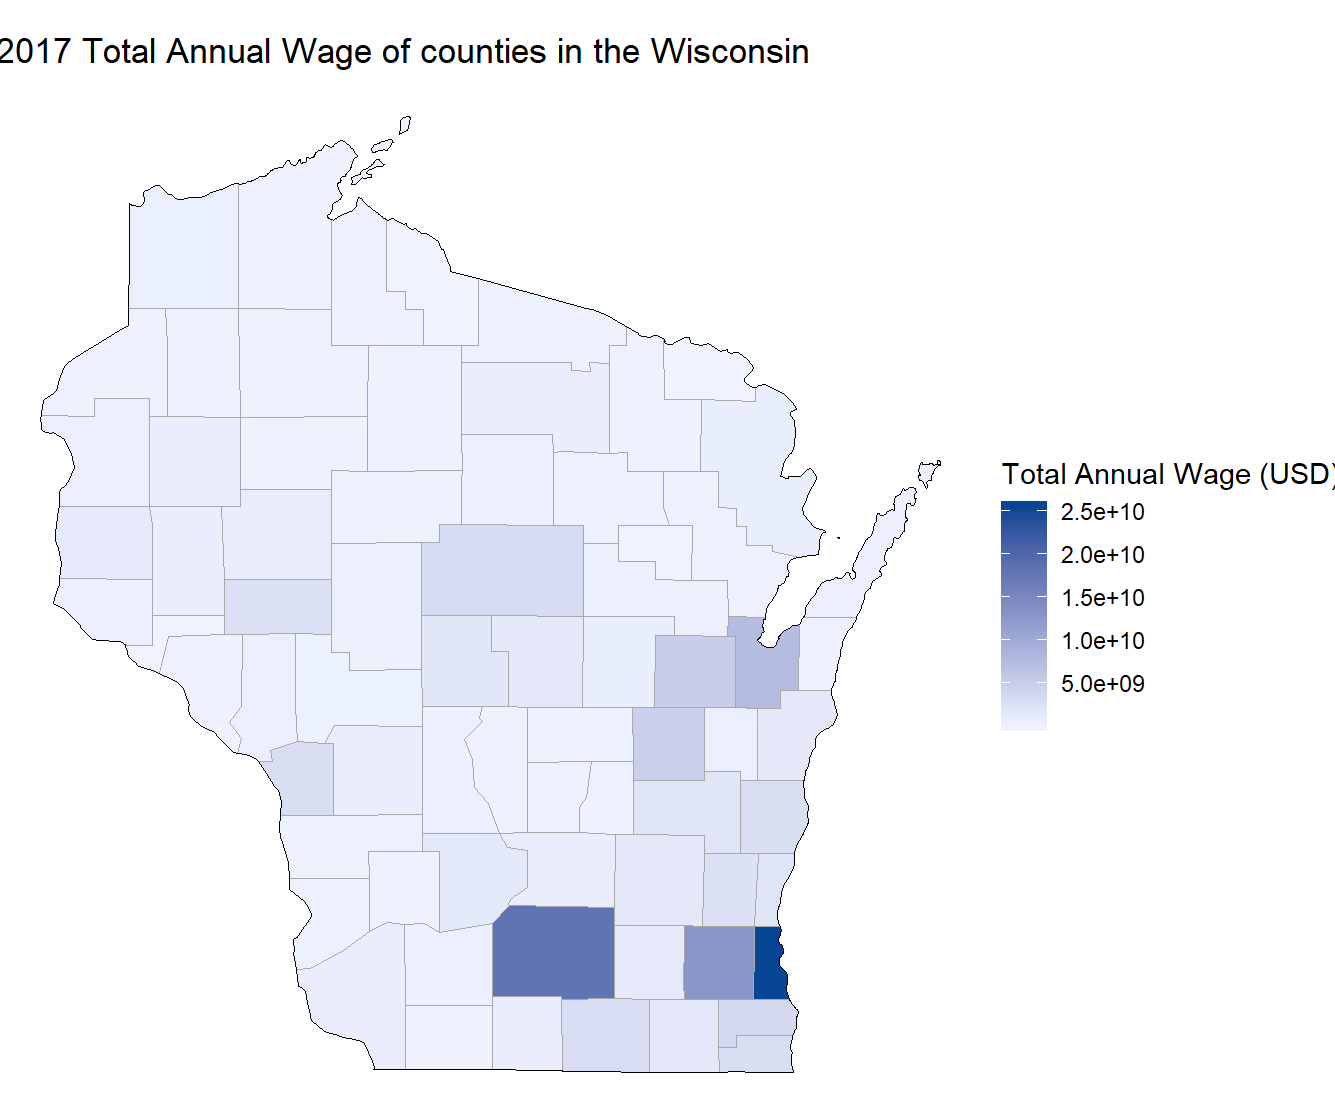
\includegraphics[width=1.0\linewidth]{2017_Total_Annual_Wage.png}
\end{center}
\caption{Plot for Total Annual Wage(Income) of counties in the Wisconsin}
\label{fig:long}
\label{fig:onecol}
\end{figure}

Seeing the plot for Total Annual Wage(Income) of counties in the Wisconsin (Fig. 1), it can be concluded that the Madison and Milwaukee area is considered as the economic center of the Wisconsin, but as this plot indicated cumulative total wage that \textbf{all} workers in each county made, it does not consider about populations of each county, which might mis-interpret the economic status of each household.

\begin{figure}
\begin{center}
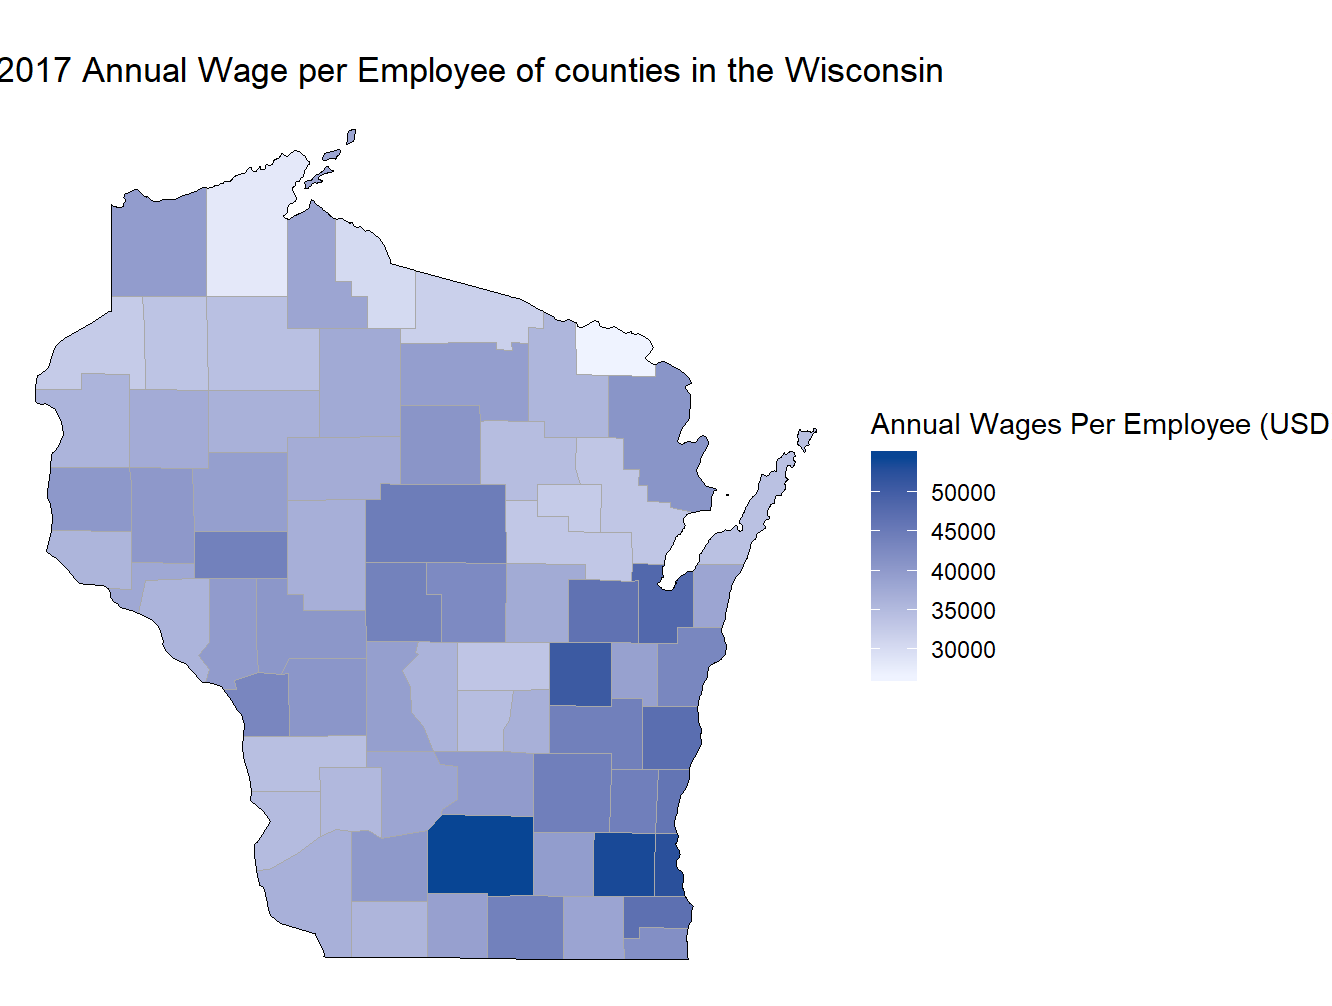
\includegraphics[width=1.0\linewidth]{2017_Annual_Wage_per_Employee.png}
\end{center}
\caption{Plot for Annual Wage(Income) per Employee of counties in the Wisconsin}
\label{fig:long}
\label{fig:onecol}
\end{figure}

Seeing the plot for Annual Wage(Income) per Employee of counties in the Wisconsin (Fig. 2), it can still be concluded that the Madison and Milwaukee area is considered as the economic center of the Wisconsin, but as this plot indicated average employee's income, it is more likely to represent household economic power compare to the previous plot.
Therefore, for further analysis, we decided to use average income to represent household economic status.

\subsection{Wisconsin Mean Income by zip code}

To get more specific data, our team decided to use dataset coded by zip code.
To begin with, we analyzed the mean income for each zip code, which indicates household economic status.

The data has been retrieved from American Community Survey (ACS), and we specifically used year 2017's census data for Mean Income In The Past 12 Months (In 2017 Inflation-Adjusted Dollars) from 2013-2017 American Community Survey 5-Year Estimates (2010, [4]).
From the cited database, we used \textbf{search criteria} below.

\begin{itemize}

\item Table Name: S1902
\item select 2017 data
\item Added Geographic after Search: 5-Digit Zip Code Tabulation Area - 860
\item state: Wisconsin
\item All 5-Digit Zip Code Tabulation Areas

\end{itemize}
\vspace{1\baselineskip}

\begin{figure}
\begin{center}
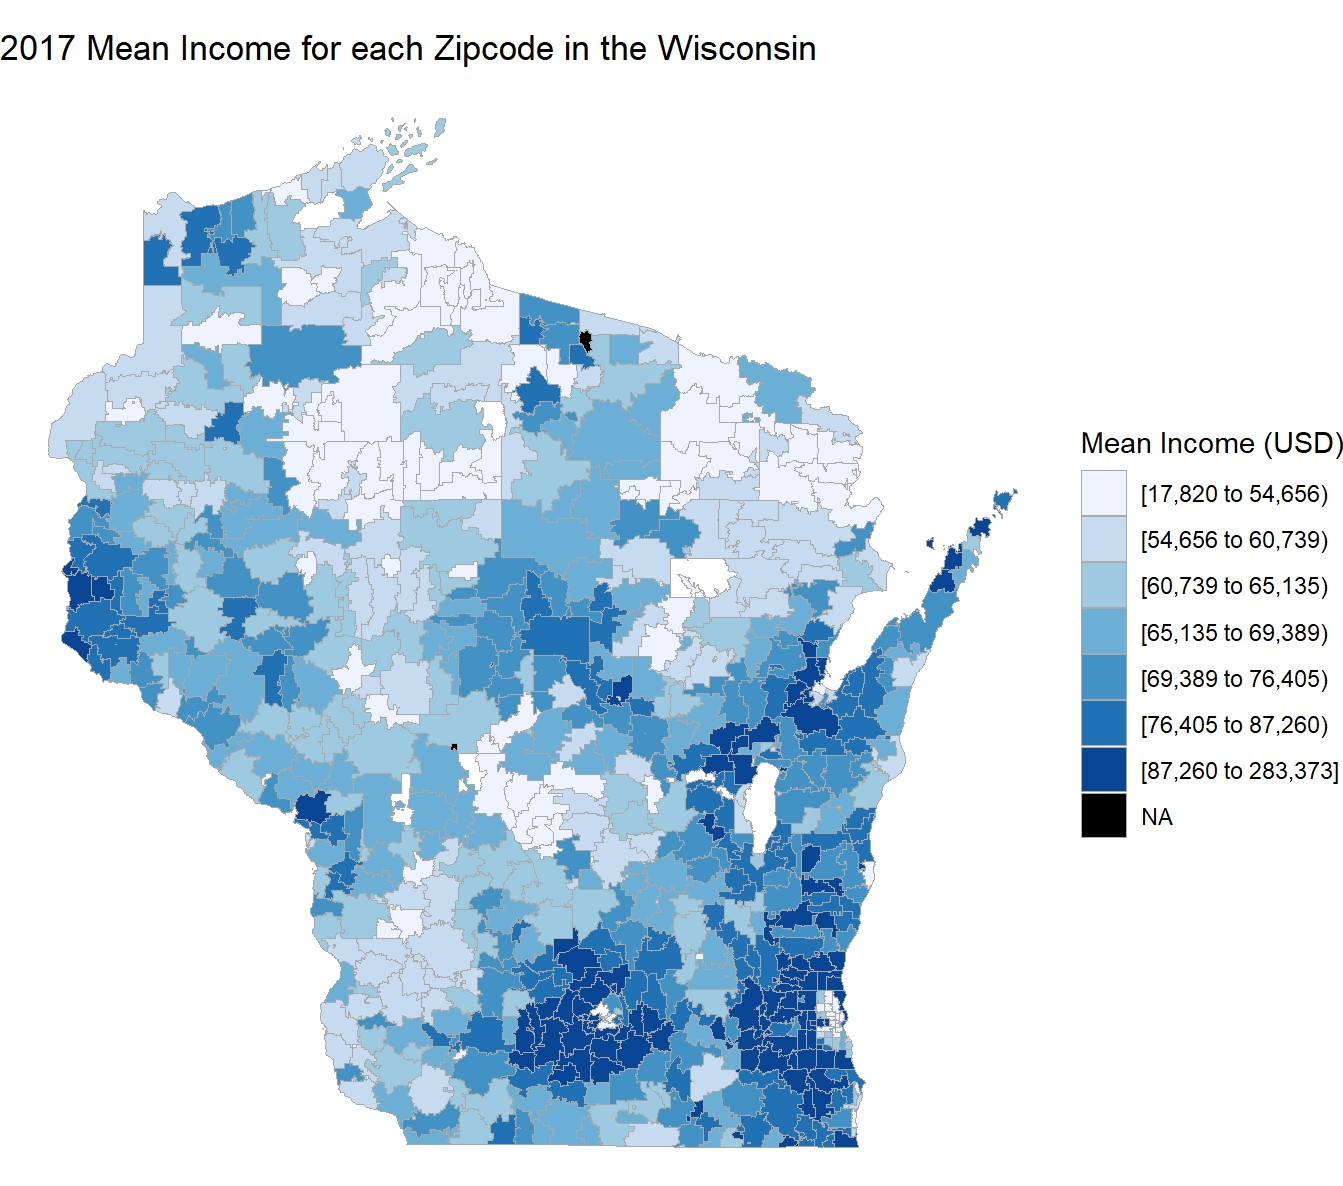
\includegraphics[width=1.0\linewidth]{2017_Mean_Income_Zipcode.jpg}
\end{center}
\caption{Plot for 2017 Mean Income for each Zip Code in the Wisconsin}
\label{fig:long}
\label{fig:onecol}
\end{figure}

By selecting Mean Income - Estimate for each zip code, we are able to get mean income for each zip code for each area.
Seeing the plot of wage coded by zip code (Fig. 3), we can still conclude that Madison and MilWaukee area's mean income is still higher than other area.
However, we are able to intuitively see that there exist outliers in this data, which does not represented in plot clearly.

Looking through the dataset, the area zip code 53047 is the outlier, where its mean income is reaching near 300 thousands.
Searched online, this zip code is belongs to Lebanon, Wisconsin, of which population is only 1664.
Concluding from this analysis, among those small number of citizens in Lebanon, on that zip code, very small number of people who earns a lot of money might live there.


\subsection{ACT Score by zip code}



\section{MATH}

Before you begin to format your paper, first write and save the content as a separate text file. Keep your text and graphic files separate until after the text has been formatted and styled. Do not use hard tabs, and limit use of hard returns to only one return at the end of a paragraph. Do not add any kind of pagination anywhere in the paper. Do not number text heads-the template will do that for you.

Finally, complete content and organizational editing before formatting. Please take note of the following items when proofreading spelling and grammar:

\subsection{Abbreviations and Acronyms} Define abbreviations and acronyms the first time they are used in the text, even after they have been defined in the abstract. Abbreviations such as IEEE, SI, MKS, CGS, sc, dc, and rms do not have to be defined. Do not use abbreviations in the title or heads unless they are unavoidable.

\subsection{Units}

\begin{itemize}

\item Use either SI (MKS) or CGS as primary units. (SI units are encouraged.) English units may be used as secondary units (in parentheses). An exception would be the use of English units as identifiers in trade, such as Ò3.5-inch disk driveÓ.
\item Avoid combining SI and CGS units, such as current in amperes and magnetic field in oersteds. This often leads to confusion because equations do not balance dimensionally. If you must use mixed units, clearly state the units for each quantity that you use in an equation.
\item Do not mix complete spellings and abbreviations of units: ÒWb/m2Ó or Òwebers per square meterÓ, not Òwebers/m2Ó.  Spell out units when they appear in text: Ò. . . a few henriesÓ, not Ò. . . a few HÓ.
\item Use a zero before decimal points: Ò0.25Ó, not Ò.25Ó. Use Òcm3Ó, not ÒccÓ. (bullet list)

\end{itemize}


\subsection{Equations}

The equations are an exception to the prescribed specifications of this template. You will need to determine whether or not your equation should be typed using either the Times New Roman or the Symbol font (please no other font). To create multileveled equations, it may be necessary to treat the equation as a graphic and insert it into the text after your paper is styled. Number equations consecutively. Equation numbers, within parentheses, are to position flush right, as in (1), using a right tab stop. To make your equations more compact, you may use the solidus ( / ), the exp function, or appropriate exponents. Italicize Roman symbols for quantities and variables, but not Greek symbols. Use a long dash rather than a hyphen for a minus sign. Punctuate equations with commas or periods when they are part of a sentence, as in

$$
\alpha + \beta = \chi \eqno{(1)}
$$

Note that the equation is centered using a center tab stop. Be sure that the symbols in your equation have been defined before or immediately following the equation. Use Ò(1)Ó, not ÒEq. (1)Ó or Òequation (1)Ó, except at the beginning of a sentence: ÒEquation (1) is . . .Ó

\subsection{Some Common Mistakes}
\begin{itemize}


\item The word ÒdataÓ is plural, not singular.
\item The subscript for the permeability of vacuum ?0, and other common scientific constants, is zero with subscript formatting, not a lowercase letter ÒoÓ.
\item In American English, commas, semi-/colons, periods, question and exclamation marks are located within quotation marks only when a complete thought or name is cited, such as a title or full quotation. When quotation marks are used, instead of a bold or italic typeface, to highlight a word or phrase, punctuation should appear outside of the quotation marks. A parenthetical phrase or statement at the end of a sentence is punctuated outside of the closing parenthesis (like this). (A parenthetical sentence is punctuated within the parentheses.)
\item A graph within a graph is an ÒinsetÓ, not an ÒinsertÓ. The word alternatively is preferred to the word ÒalternatelyÓ (unless you really mean something that alternates).
\item Do not use the word ÒessentiallyÓ to mean ÒapproximatelyÓ or ÒeffectivelyÓ.
\item In your paper title, if the words Òthat usesÓ can accurately replace the word ÒusingÓ, capitalize the ÒuÓ; if not, keep using lower-cased.
\item Be aware of the different meanings of the homophones ÒaffectÓ and ÒeffectÓ, ÒcomplementÓ and ÒcomplimentÓ, ÒdiscreetÓ and ÒdiscreteÓ, ÒprincipalÓ and ÒprincipleÓ.
\item Do not confuse ÒimplyÓ and ÒinferÓ.
\item The prefix ÒnonÓ is not a word; it should be joined to the word it modifies, usually without a hyphen.
\item There is no period after the ÒetÓ in the Latin abbreviation Òet al.Ó.
\item The abbreviation Òi.e.Ó means Òthat isÓ, and the abbreviation Òe.g.Ó means Òfor exampleÓ.

\end{itemize}


\section{USING THE TEMPLATE}

Use this sample document as your LaTeX source file to create your document. Save this file as {\bf root.tex}. You have to make sure to use the cls file that came with this distribution. If you use a different style file, you cannot expect to get required margins. Note also that when you are creating your out PDF file, the source file is only part of the equation. {\it Your \TeX\ $\rightarrow$ PDF filter determines the output file size. Even if you make all the specifications to output a letter file in the source - if your filter is set to produce A4, you will only get A4 output. }

It is impossible to account for all possible situation, one would encounter using \TeX. If you are using multiple \TeX\ files you must make sure that the ``MAIN`` source file is called root.tex - this is particularly important if your conference is using PaperPlaza's built in \TeX\ to PDF conversion tool.

\subsection{Headings, etc}

Text heads organize the topics on a relational, hierarchical basis. For example, the paper title is the primary text head because all subsequent material relates and elaborates on this one topic. If there are two or more sub-topics, the next level head (uppercase Roman numerals) should be used and, conversely, if there are not at least two sub-topics, then no subheads should be introduced. Styles named ÒHeading 1Ó, ÒHeading 2Ó, ÒHeading 3Ó, and ÒHeading 4Ó are prescribed.

\subsection{Figures and Tables}

Positioning Figures and Tables: Place figures and tables at the top and bottom of columns. Avoid placing them in the middle of columns. Large figures and tables may span across both columns. Figure captions should be below the figures; table heads should appear above the tables. Insert figures and tables after they are cited in the text. Use the abbreviation ÒFig. 1Ó, even at the beginning of a sentence.

\begin{table}[h]
\caption{An Example of a Table}
\label{table_example}
\begin{center}
\begin{tabular}{|c||c|}
\hline
One & Two\\
\hline
Three & Four\\
\hline
\end{tabular}
\end{center}
\end{table}


   \begin{figure}[thpb]
      \centering
      \framebox{\parbox{3in}{We suggest that you use a text box to insert a graphic (which is ideally a 300 dpi TIFF or EPS file, with all fonts embedded) because, in an document, this method is somewhat more stable than directly inserting a picture.
}}
      %\includegraphics[scale=1.0]{figurefile}
      \caption{Inductance of oscillation winding on amorphous
       magnetic core versus DC bias magnetic field}
      \label{figurelabel}
   \end{figure}
   

Figure Labels: Use 8 point Times New Roman for Figure labels. Use words rather than symbols or abbreviations when writing Figure axis labels to avoid confusing the reader. As an example, write the quantity ÒMagnetizationÓ, or ÒMagnetization, MÓ, not just ÒMÓ. If including units in the label, present them within parentheses. Do not label axes only with units. In the example, write ÒMagnetization (A/m)Ó or ÒMagnetization {A[m(1)]}Ó, not just ÒA/mÓ. Do not label axes with a ratio of quantities and units. For example, write ÒTemperature (K)Ó, not ÒTemperature/K.Ó

\section{CONCLUSIONS}

A conclusion section is not required. Although a conclusion may review the main points of the paper, do not replicate the abstract as the conclusion. A conclusion might elaborate on the importance of the work or suggest applications and extensions. 

\addtolength{\textheight}{-12cm}   % This command serves to balance the column lengths
                                  % on the last page of the document manually. It shortens
                                  % the textheight of the last page by a suitable amount.
                                  % This command does not take effect until the next page
                                  % so it should come on the page before the last. Make
                                  % sure that you do not shorten the textheight too much.

%%%%%%%%%%%%%%%%%%%%%%%%%%%%%%%%%%%%%%%%%%%%%%%%%%%%%%%%%%%%%%%%%%%%%%%%%%%%%%%%



%%%%%%%%%%%%%%%%%%%%%%%%%%%%%%%%%%%%%%%%%%%%%%%%%%%%%%%%%%%%%%%%%%%%%%%%%%%%%%%%



%%%%%%%%%%%%%%%%%%%%%%%%%%%%%%%%%%%%%%%%%%%%%%%%%%%%%%%%%%%%%%%%%%%%%%%%%%%%%%%%
\section*{APPENDIX}

Appendixes should appear before the acknowledgment.

\section*{ACKNOWLEDGMENT}

The preferred spelling of the word ÒacknowledgmentÓ in America is without an ÒeÓ after the ÒgÓ. Avoid the stilted expression, ÒOne of us (R. B. G.) thanks . . .Ó  Instead, try ÒR. B. G. thanksÓ. Put sponsor acknowledgments in the unnumbered footnote on the first page.



%%%%%%%%%%%%%%%%%%%%%%%%%%%%%%%%%%%%%%%%%%%%%%%%%%%%%%%%%%%%%%%%%%%%%%%%%%%%%%%%

References are important to the reader; therefore, each citation must be complete and correct. If at all possible, references should be commonly available publications.



\begin{thebibliography}{99}

\bibitem{c1} Rugaber, C. S. (2017, January 12). Pay gap between college grads and everyone else at a record. Retrieved November 27, 2019, from https://www.usatoday.com/story/money/2017/01/12/pay-gap-between-college-grads-and-everyone-else-record/96493348/.

\bibitem{c2} QCEW News Releases. (n.d.). Retrieved December 2, 2019, from https://www.bls.gov/cew/.

\bibitem{c3} Data Slices by Industry. (2016, June 21). Retrieved December 2, 2019, from \newline
https://data.bls.gov/cew/doc/access/csv\_data\_slices.htm\#ANNUAL\_LAYOUT.

\bibitem{c4} American FactFinder - Search. (2010, October 5). Retrieved December 2, 2019, from \newline https://factfinder.census.gov/faces/nav/jsf/pages/searchresults.xhtml?refresh=t.

\end{thebibliography}




\end{document}
